\section{Basic Antenna Theory and HFSS Simulations}
Even today, a full 140 years after the publication of 
Maxwell's \textit{Treatise on Electricity and Magnetism}, 
the electromagnetic modeling of radiating structures 
is an ongoing research problem. The notorious difficulty 
of solving Maxwell's equations seriously hampers analy\-ti\-cal efforts
and, due to the nature of electromagnetic radiation, numerical
progress is not easier to achieve.

In what follows, we present the basic equations of 
antenna theory (Maxwell's) and discuss the nature 
of sources in this framework (currents and charges). 

\subsection{Maxwell's Equations}
Being, by now, comfortable with the basic form of Maxwell's equations, 
we will simply state them for linear, non-chiral and reciprocal media
and allow for the existence of current and charge densities. 
They are (in Lorentz-Heaviside units with $c=1$) \cite{NOV2012}
  \begin{subequations}
  \begin{align}
   \nabla\times\bo{E}+\frac{\partial(\mu\bo{H})}{\partial t}	&=0	\\
   \nabla\times\bo{H}-\frac{\partial(\epsilon\bo{E})}{\partial t}-\bo{J}_c&=\bo{J}_s\\
   \nabla\cdot(\epsilon\bo{E})					&=\rho	\\
   \nabla\cdot(\mu\bo{H})					&=0
  \end{align}
  \end{subequations}
where we have separated the current using two terms: a source current, $\bo{J}_s$ and
an induced conduction current $\bo{J}_c$. The induced conduction current
is related to the electric field via Ohm's law, i.e.
  \begin{equation}
   \bo{J}_c=\sigma\bo{E}
  \end{equation}
while the source current is a prepared, physical source initially 
independant of the system.

A technical point is in order. In the antenna literature, the induced
currents and charge density are considered as the fundamental quantities 
that \textit{produce} the fields. While worthwhile (see the Stratton-Chu section), 
this viewpoint requires that either (i) we have \textit{a priori} knowledge of 
the sources ($\bo{J}_t=\bo{J}_c+\bo{J}_s$ and $\rho$) or (ii) that we use the
constitutive relations down the line. The first case applies to situations
where the induced current is trivially known (e.g. the dipole antenna) or
when $\sigma=0$ and $\bo{J}_s$ is known.

Also, even though the $\bo{H}$ field was introduced as an auxiliary field to take
into account the effect of an applied magnetic field to the material, we 
take it as the fundamental field as it leads to more easily solvable
equations and is a completely equivalent choice. 

\subsection{Stratton-Chu Solution}
In antenna problems, we want to compute the field values as a function of 
the sources that contribute to these fields. From electrostatics, we know 
that a current density $\bo{J}$ gives rise to an electric field and a charge 
density $\rho$ gives rise to a magnetic field. In the time-varying picture, 
the electric and magnetic fields become coupled and we take the viewpoint that
the $\bo{J}$ and $\rho$ give rise to both electric and magnetic fields. 

To compute the field from these sources, which are presupposed to exist, 
we must use the Stratton-Chu integrals. The derivation is standard, so we 
refer to \cite{ELL2003}. Consider a volume $V$ of free space containing
sources and possibly excluded subvolumes $V_i$ bound by surfaces $S_i$ that contain matter
of some kind. By the use of Green's and Stokes' theorems and other vectorial 
identities, we find that the field outside the excluded subvolumes
can be expressed as
  \begin{align}
   \bo{E} &= \frac{1}{4\pi}\mathop{\iiint}_V \left(\rho\nabla G+i\omega G\bo{J}\right)dV
	+\frac{1}{4\pi}\oiint_{S_1,\cdots,S_N}\left[\bo{n}\cdot\bo{E}\nabla G+(\bo{n}\times\bo{E})\times\nabla G+i\omega G(\bo{n}\times\bo{H})\right]dS\label{eq:antenna.strattonChuE}\\
   \bo{H} &= \frac{1}{4\pi}\mathop{\iiint}_V \bo{J}\times\nabla G dV
	+\frac{1}{4\pi}\oiint_{S_1,\cdots,S_N}\left[-i\omega G(\bo{n}\times\bo{E})+(\bo{n}\times\bo{H})\times\nabla G+(\bo{n}\cdot\bo{H})\nabla G\right]dS\label{eq:antenna.strattonChuH}
  \end{align}
where $G$ is the Green's function of the problem
  \begin{equation}
   G(\bo{r},\bo{r}') = \frac{e^{ik|\bo{r}-\bo{r'}|}}{4\pi|\bo{r}-\bo{r}'|}.
  \end{equation}

These two equations are rigorous solutions of Maxwell's equations. 
They can be used with any antenna and provide ways to compute the 
current distribution if is unknown (constitutes an integral equation in the current)
and can be used to compute the far-field of antennae when either 
(i) the current distribution is known or (ii) the near-field around the antenna
is known. 
These two properties discriminate antennae into two categories, denoted Type I and Type II.

Type I antennae have a well-approximated current distribution, which means that there are no
subvolumes to be excluded and therefore no surface integrals in expressions 
\eqref{eq:antenna.strattonChuE} and \eqref{eq:antenna.strattonChuH}. 

On the other hand, Type II antennae have well-approximated near-fields, leading
us to exclude the volume containing the antenna. Expressions \eqref{eq:antenna.strattonChuE}
and \eqref{eq:antenna.strattonChuH} contain only surface integrals, then. 

\subsection{Antenna Parameters}
In the design of our antenna, we will want to optimize the value
of some parameters. We will now describe some of these parameters.

\subsubsection[Directivity and Gain]{Directivity and Gain \cite[\S 1.16]{ELL2003}}
Given a radiation pattern measured (in the far-field) as the power density 
$\mathcal{P}(\theta,\varphi)$, we can define its \textit{directivity}
as
  \begin{equation}
   D(\theta,\varphi) = \frac{4\pi\mathcal{P}(\theta,\varphi)}
			{\int_0^\pi\int_0^{2\pi}\mathcal{P}(\theta',\varphi')\sin\theta'd\theta'd\varphi'}.
  \end{equation}
The value of the directivity is less than unity if the power density radiated at angle $(\theta,\varphi)$
is less than the average power radiated. For instance, an isotropic antenna will possess a unit directivity
for all angles while a highly directional antenna will have a sharp peak  in its directivity function 
at some angle $(\theta,\varphi)$.

Another interesting concept to introduce is \textit{partial directivity}. 
The power density can be divided into two contributions: the $\theta$-polarized
and the $\varphi$-polarized polarization and we can write
  \begin{equation}
    \mathcal{P}(\theta,\varphi) = \mathcal{P}_\theta(\theta,\varphi)+\mathcal{P}_\varphi(\theta,\varphi)
  \end{equation}
where the subscripts indicate the polarization state. The partial 
directivities hence follow
  \begin{equation}
   D(\theta,\varphi) = D_\theta(\theta,\varphi)+D_\varphi(\theta,\varphi).
  \end{equation}

We can also introduce the gain, which characterizes the loss
and the directivity of the antenna simultaneously. It is simply given
as
  \begin{equation}
    G(\theta,\varphi) = \frac{4\pi r^2\mathcal{P}(\theta,\varphi)}{P}
  \end{equation}
where $P$ is the power accepted by the antenna. Because of the 
losses, $P/r^2>\int_0^\pi\int_0^{2\pi}\mathcal{P}(\theta',\varphi')\sin\theta'd\theta'd\varphi'$
such that $G(\theta,\varphi)<D(\theta,\varphi)$. 

We can also define partial gains in the exact same fashion we defined partial
directivities.

Radiation efficiency $\eta$ is defined as the ratio of the total radiated power 
to the power accepted by the antenna \cite{IEEE145-1993}.

\subsubsection{Scattering Parameters}
The scattering parameters (or $S$-parameters) are
usually defined through a linear $N$-port network. 
Suppose we have an electronic device comprising
$N$ ports, or points of entry. Imagine shining light onto
one of the ports, say port $j$. A certain percentage
of the power carried by this light be reflected 
by this port and the rest will be transmitted to the
other ports or absorbed in the medium. The \textit{reflection}
coefficient is given by $S_{jj}$ while the transmission
coefficients are given $S_{ji}$ ($i\neq j$) where $\mat{S}$
is the scattering matrix of the network. In a reciprocal (in the sense
of Lorentz) network, the scattering matrix will be equal to its
transpose, i.e. $S_{ij}=S_{ji}$. In a lossless network, the scattering
matrix will be unitary. 

This is, of course, highly reminiscent of the scattering operator
in quantum-mechanical scattering which relates the outgoing (scattered)
components to the incoming (incident) components
  \begin{equation}
   \Ket{\Psi_\text{out}}=\mathcal{S}\Ket{\Psi_\text{in}}.
  \end{equation}
In this case, the ``ports'' are the different angular momenta
components rather than physical input/output connections. 
Ports are somewhat arbitrary in optical structures.

\subsection{HFSS Simulations of an LCX Antenna}
In our quest of finding a fibre-antenna design that can easily be integrated into
textile, we have stumbled upon the leaky coaxial cable (LCX) design: a basic coaxial cable
from which are cut windows as to expose the dielectric core. The radiation characteristics
can be tuned by changing the geometric properties of the windows. 

LCX antennae are usually analyzed using harmonic analysis \cite{WAN2001}. 
In our case, however, we cannot consider the structure to be periodic, as the total 
length of the fibre-antenna is of the order of the wavelength ($\lambda\sim12\unit{cm}$) and the period
of the slots is smaller than the wavelength. Moreover, given the size of the slots, 
the author is comfortable to say that we neither are in the perturbation regime. 
Figure \ref{fig:antenna.fibre-antenna} shows the actual design and the important parameters.

Given the wild scale in the size of the structures (from the nanometer to the millimeter), we use
the FEM to solve the driven problem. The parameters of interest will be the scattering parameters, the
radiation pattern and antenna efficiency, gain and directivity. We will first model the fibre-antennae
that were fabricated. There will be a subsequent optimization phase.

\subsubsection{Preliminary Results}
We first model the RF21 design. Its parameters are summarized in 
Table \ref{tab:antenna.rfxx-parameters}. 

Notice the small thickness
of the silver layers (126 and 101 nm) compared to the other 
sizes involved. It takes a highly non-uniform mesh to model
these small relative sizes. Moreover, since the silver has a high
conductivity, it takes an even smaller mesh to model. Our first 
attempts at modeling this structure proved unsuccessful.

In the experimental data (\see Figure \ref{fig:antenna.sParameters}), 
we see deep dips in the transmission spectrum ($S_{12}$) at approximately
1.8 GHz and 3 GHz. There are corresponding dips in the reflection parameters,
$S_{11}$ and $S_{22}$, which leads us to believe that remaining power 
was radiated through the slots. The existence of two dips seems predicated on the asymmetry
of the fibre ($d_L\neq d_R$). 

We also notice that the simulation data does not in any way correlate
to the experimental data. This is probably due to the fact that, in the our
HFSS model, we had to put the thickness of the silvers layers to $2\,\unit{\mu m}$
instead of the values listed in Table \ref{tab:antenna.rfxx-parameters}. In 
this regime, the fibre-antenna behaves like an ordinary transmission line. 
However, as the mesher does not allow us to go under $2\,\unit{\mu m}$, we cannot
conclude that is really due to the thickness of the Ag layers, only suspect it.

In our following report, we will break down the problem
to make it analytically tractable and try to analyze the effect of ``small''
silver layers on the propagation of light. 

\begin{figure}
 \begin{center}
 \begin{tikzpicture}
  % -- Draw the overall shape.
  \draw[very thick] (0,0) -- (8,0) -- ++(0,-2) -- ++(-3,0) -- ++(0,-2) -- ++(-2,0) -- ++(0,2) -- ++(-3,0) -- ++(0,2); 
  
  % -- We draw the reflected/transmitted arrows.
  \draw[->,>=stealth] (8.25,-0.5) -- ++(1,0) node[near end,above] {$a_1$};
  \draw[<-,>=stealth] (8.25,-1.5) -- ++(1,0) node[near end,above] {$b_1$};
  \draw[<-,>=stealth] (-1.25,-0.5) -- ++(1,0) node[near start,above] {$a_2$};
  \draw[->,>=stealth] (-1.25,-1.5) -- ++(1,0) node[near start,above] {$b_2$};
  \draw[->,>=stealth] (3.5,-4.25) -- ++(0,-1) node[near end,right] {$a_3$};
  \draw[<-,>=stealth] (4.5,-4.25) -- ++(0,-1) node[near end,right] {$b_3$};
 \end{tikzpicture}
 \end{center}
 \caption[Example of a 3-port network]{Example of a 3-port network. The ``ends'' of the structure are generally used at its ports.}
 \label{fig:antenna.network}
\end{figure}

\begin{figure}
 \centering
 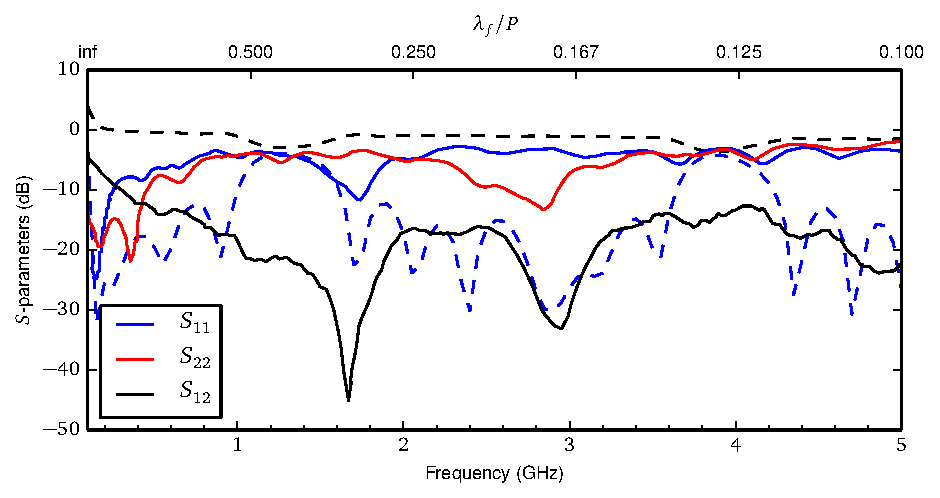
\includegraphics[width=\textwidth]{figs/active/sParametersRF21.pdf}
 \caption[$S$-parameters of the RF21 fibre design]{$S$-parameters of the RF21 fibre design. The full lines represent
	  the experimental data while the dotted lines represent the simulation data.
	  The top $x$ axis shows the $S$-parameters as a function of the ratio of the 
	  vacuum wavelength $\lambda_f$ over the period of the windows $P$.}
 \label{fig:antenna.sParameters}
\end{figure}

